\section{Implementation}

\subsection{Code Style Configuration}
\begin{frame}
\frametitle{Code Style Configuration}

The measurement component enforces some code styles:

\begin{itemize}
  \item Indentation levels
  \item Import statement styles
  \item Method name format
\end{itemize}

The code style is configurable using a JSON file:

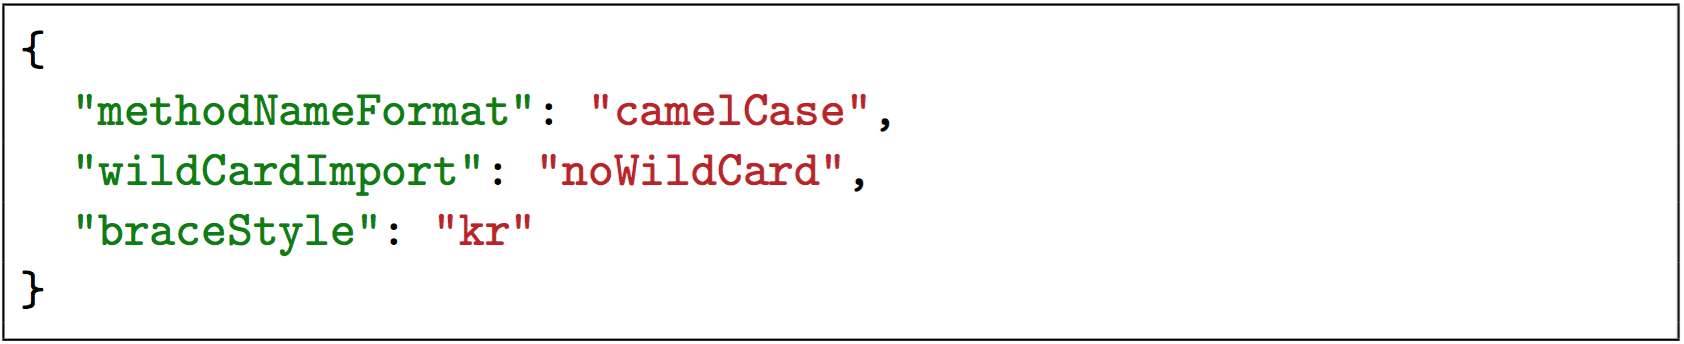
\includegraphics[scale=0.37]{json_config}

\end{frame}

\begin{frame}
\frametitle{Code Style Configuration}

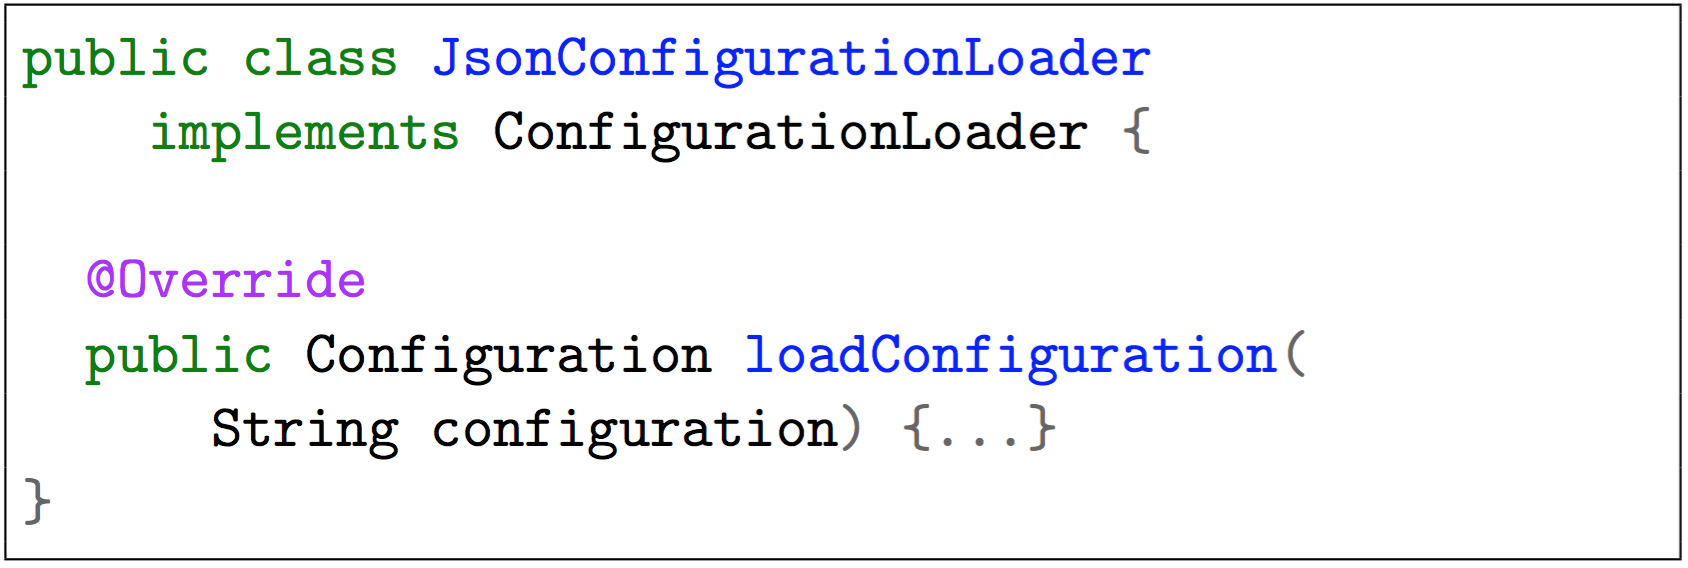
\includegraphics[scale=0.37]{json_configuration_loader}

\only<1>{
Measurement component uses \textit{JsonConfigurationLoader} to convert the configuration in \textit{String} to \textit{Configuration} object.
}

\only<2>{
We can implement the \textit{ConfigurationLoader} to support configuration XML and CSV formats.
}
\end{frame}

\subsection{Score Calculator}
\begin{frame}
\frametitle{Score Calculator}
\setbeamercovered{transparent}

\begin{columns}
\column{0.5\textwidth}
Washizaki et al. (2007) calculate scores based on \emph{benchmark} values and \emph{collected} values by using a linear piecewise function:
\begin{itemize}
  \item<1,4> If the collected value is less than benchmark value, the score is 100\%
  \item<2,4> If the collected value is more than benchmark value and less than 3 times of benchmark, the score is: $$score=\bigg(-\frac{1}{3 \times benchmark} \times value + \frac{4}{3}\bigg) \times 100\%$$
  \item<3,4> Else, the score is zero
\end{itemize}

\column{0.5\textwidth}
\begin{tikzpicture}
\begin{axis}[
    axis lines = left,
    xlabel = value,
    ylabel = score,
]
\addplot [
    domain=1:4, 
    samples=2,
    color=red,
]
{- x/3 + 4/3 };
\addplot [
    domain=0:1, 
    samples=2,
    color=red,
]
{1};
\addplot [
    domain=4:5, 
    samples=2,
    color=red,
]
{0};
\addplot [
    domain=0:1, 
    samples=2, 
    color=white,
]
{1.1};
\end{axis}
\end{tikzpicture}

\end{columns}

\end{frame}